\section{Secure User Interaction}


Web-based interfaces are very prevalent to remotely configure safety-critical systems such as remote PLCs~\cite{controlbyweb} or medical devices~\cite{medicalDevice}, and other security-sensitive applications such as online payments, e-voting, etc. The high complexity of modern operating systems, software, and hardware components has shown that computer systems largely remain vulnerable to attacks. A compromised computer threatens the integrity and the confidentiality of any interaction between the user and a remote server. It can easily alter the data exchanged between the user and the remote server, trick the user to perform unintended actions, or observe any sensitive IO data. 


\emph{Trusted path} provides a secure channel between the user (specifically human interface device - HID) and the end-point, which is typically a trustworthy application running on the host. Trusted path ensures that user inputs reach the intended application unmodified, and all the outputs presented to the user are generated by the legitimate application. Trusted path to the local host is a well-researched area where many solutions focus on using trusted software components such as a trusted hypervisor. Zhou et al.~\cite{zhou2012building} proposed a generic trusted path on $x86$ systems with a pure hypervisor-based design. SGXIO~\cite{weiser2017sgxio} employs both a hypervisor and Intel SGX. However, hypervisors are hard to deploy, have a large TCB, and are impractical in real-world scenarios as most of the existing verified hypervisors offer a minimal set of features. 

\subsection{Limitations in the Current TEE}

The recent introduction of trusted computing architectures like Intel's SGX has enabled secure computations and secure data storage on otherwise untrusted computing platforms. However, such architectures do not directly enable secure user interaction because IO operations are handled by the operating system. Additionally, the recent microarchitectural attacks have shown that execution environments inside enclaves, like the one provided by SGX, can be compromised as well.


\subsection{External Hardware and Related Solutions}

Trusted external devices are another way to realize secure IO between a user and a remote server. Transaction confirmation devices~\cite{filyanov2011uni,weigold2011secure} allow the user to review her input data on a trusted device that is physically separated from the untrusted host. These approaches suffer from poor usability, security issues due to user habituation and are only limited to simple inputs. Bump in the Ether~\cite{McCPerRei2006} and IntegriKey~\cite{IntegriKey} use external embedded devices to sign input parameters. However, such solutions do not support output integrity; hence, the attacker can execute UI manipulation attacks to trick the user into providing incorrect inputs. Trusted overlay-based approach~\cite{brandon2017trusted} uses a trusted FPGA to overlay UI elements such as a PIN entry screen on the LCD where the user can safely enter passwords. The approach has several drawbacks - i) lack of support for UI elements apart from text field, ii) there is no way for the user to distinguish attacker-rendered UI from the trusted overlaid UI, iii) lack of mouse support, and iv) lack of integration with applications such as browsers.


Fidelius~\cite{Fidelius} combines the previous ideas of Bump in the Ether and trusted overlay to protect keyboard inputs from a compromised browser using external devices and a \js interpreter that runs inside an SGX enclave. Fidelius maintains overlays on display, specifically on the input text boxes to hide sensitive user inputs from the browser. We investigate the security of Fidelius and discover several issues. Fidelius imposes a high cognitive load to the users as they need to monitor continuously different security indicators (two LED lights and the status bar on the screen) to guarantee the integrity and confidentiality of the input. Furthermore, the attacker can manipulate labels of the UI elements to trick the user into providing incorrect input. 
The lack of mouse support, which may appear only as functional limitation, exposes Fidelius to early form submission attacks. The host can emulate a mouse click on the submit button before the user completes all fields of a form.
%Not supporting mouse, may appear only as a functional limitation, but it exposes Fidelius to early form submission attack where the host can emulate a mouse click on the submit button while the user is in the process of typing into a text field. 
This allows the attacker to perform an early form submission with incomplete input - a violation of input integrity. Fidelius is also vulnerable to microarchitectural attacks on SGX enclaves~\cite{van2018foreshadow} that extract attestation keys and relay attacks~\cite{dhar2018proximitee} that relay all user data to the attacker's platform.

The drawbacks of the existing systems show that ensuring the integrity and confidentiality of the IO in the presence of an untrusted host is a non-trivial problem and requires a comprehensive solution. All of the previous trusted path solutions neither protect both input and output simultaneously, nor do they consider different modalities of input.



\subsection{Requirements of Security and Functional Properties}
\label{goals}

The lack of security properties and features in the existing solutions provides the necessary security and functional requirements for a trusted path that provides IO integrity and confidentiality and is usable. We can now summarize the observations that we derived from the literature as following:

\myparagraph{R1. Inter-dependency between input and output} 
The first and second observations from the existing solutions show that the output and input security depend on each other, and they should be considered together. Otherwise, the attacker can manipulate the output to influence the user input.
%The main lesson that we learn from the previous papers is that input and output integrity, and confidentiality cannot be considered in isolation. Rather, they are needed to be secured simultaneously as the output, and the input both influence each other.  

\myparagraph{R2. Inter-dependency between all input modalities} 
Existing web interfaces allow users to complete forms by using different modalities for the user input, namely the keyboard, the mouse, and the touchpad. The third observation shows that a secure system should protect simultaneously all user input modalities to achieve input integrity (against early-form submission and clickjacking).

%If there exist multiple input sources (typically keyboard and mouse), all of them should be protected simultaneously as these input sources influence each other. For example, in a web application scenario, protecting the integrity of only the keyboard input does not provide input integrity as an attacker-controlled host can always execute an early form submission attack.

\myparagraph{R3a. No cognitive load for IO integrity} 
A system that protects IO operations should introduce minimal or no cognitive load to its users for input integrity.
The system should guarantee the output integrity of the legitimate information necessary to complete a form and avoid asking the user to interact with an external device or monitor security indicators out-of-context.

%Output integrity protection can eliminate the actions that lead to high cognitive loads to the user.  Such as using an external device to confirm every transaction, looking to a passive security indicator and confirming actions, etc. The systems that rely heavily on such security measures suffer from input errors that originate from user habituation. Moreover, such designs require user training that makes the system hard to deployment and costly.

\myparagraph{R3b. User attention for IO confidentiality} Preserving the confidentiality of user inputs against a compromised host is a challenging task because the host can trick the user to reveal her inputs when the system is not active. Therefore, requiring users to perform a small action, e.g., press a key, before entering confidential inputs is a valid trade-off between usability and security.

%Confidentiality requires active triggering from the user to distinguish the secure part of the screen from ensuring part of the screen if the part of the output provides integrity/confidentiality protection.

\myparagraph{R4. Small trust assumptions and deployability} 
Our goal is to provide the rich set of IO and security features with minimal trust assumptions that do not rely on a trusted OS, specialized hypervisor, or TEEs such as Intel SGX. Preferably, the solution should be easy to set up for users, i.e., plug-and-play, and integrate well with the existing infrastructure.  




\subsection{System Overview}

\begin{figure}[t]
\centering
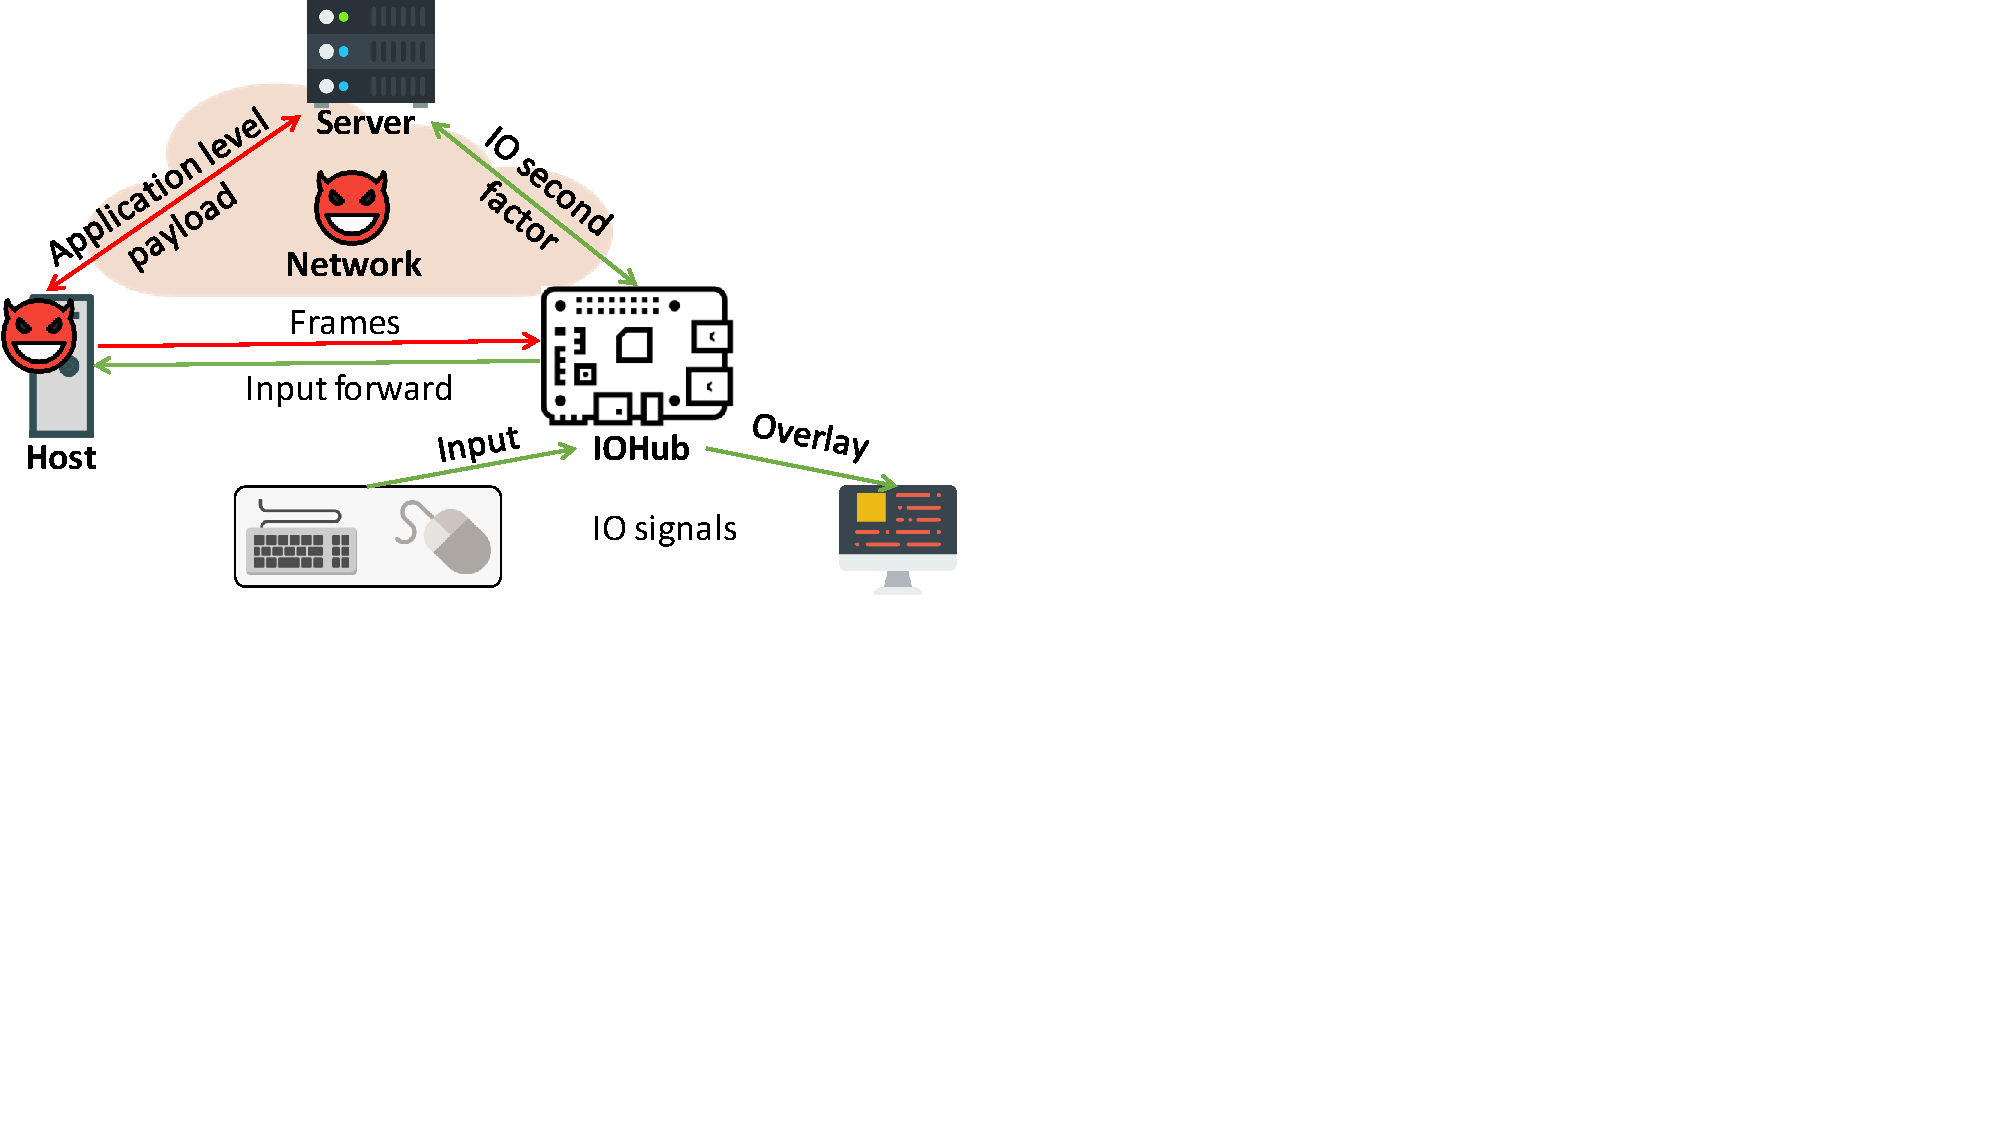
\includegraphics[trim={0 8.5cm 17cm 0}, clip, width=0.85\linewidth]{approachOverview.pdf}
\caption{\textbf{High-level approach overview of our solution.}  The \device connects the trusted IO devices and the attacker-controlled host. 
}
\spacesave
\label{fig:approachOverview}
\centering
\end{figure}


In this section, we present an overview of our solution: \name. On the high-level, \name uses the concept of the \emph{bump in the wire} (such as bump in the ether~\cite{McCPerRei2006}) to provide integrity and confidentiality to the user IO{}s between the IO devices and the remote server. \name achieves this by utilizing a trusted embedded device as a mediator between all the IO devices and the untrusted host.  We call this trusted intermediary \device for the rest of this paper.   


\subsubsection{System and Attacker Model}

We consider a typical scenario where the user wants to interact with a trusted remote web server via an attacker-controlled host. The model is depicted in Figure~\ref{fig:approachOverview} which shows the untrusted host, the remote server, and the user IO devices. We only assume that the monitor, keyboard, mouse (in a word all the IO devices that we need to protect from the malicious host) and the \device are trusted. The \device works as a mediator between all the IO devices and the host. Note that the \device has no network capability to communicate with the server directly, rather it relies on the host and uses it as an untrusted transport. We also assume that the \device comes with preloaded certificates and keys that allow the \device to verify the signatures signed by the server and sign data such as the user input.

There are many possible ways to deploy \name. One way is to assume that the \device manufacturer issues a certificate for each of the deployed \device{}s . The \device maintains a whitelist for the remote servers along with their public certificates. This allows the \device to verify messages signed by those remote servers. Another assumption could be that the \device is issued by a service provider who also runs the remote server. 

\myparagraph{Attacker model and capabilities} Our attacker model assumes that the host (OS, installed applications, and hardware) and the network are attacker-controlled. The attacker can intercept, and arbitrarily manipulate (such as create, drop, or modify) the user IO data between the user and the remote server. Furthermore, we assume that the attacker can not break the physical security of the \device.



\subsection{High-level Description of the System}

\begin{figure}[t]
\centering
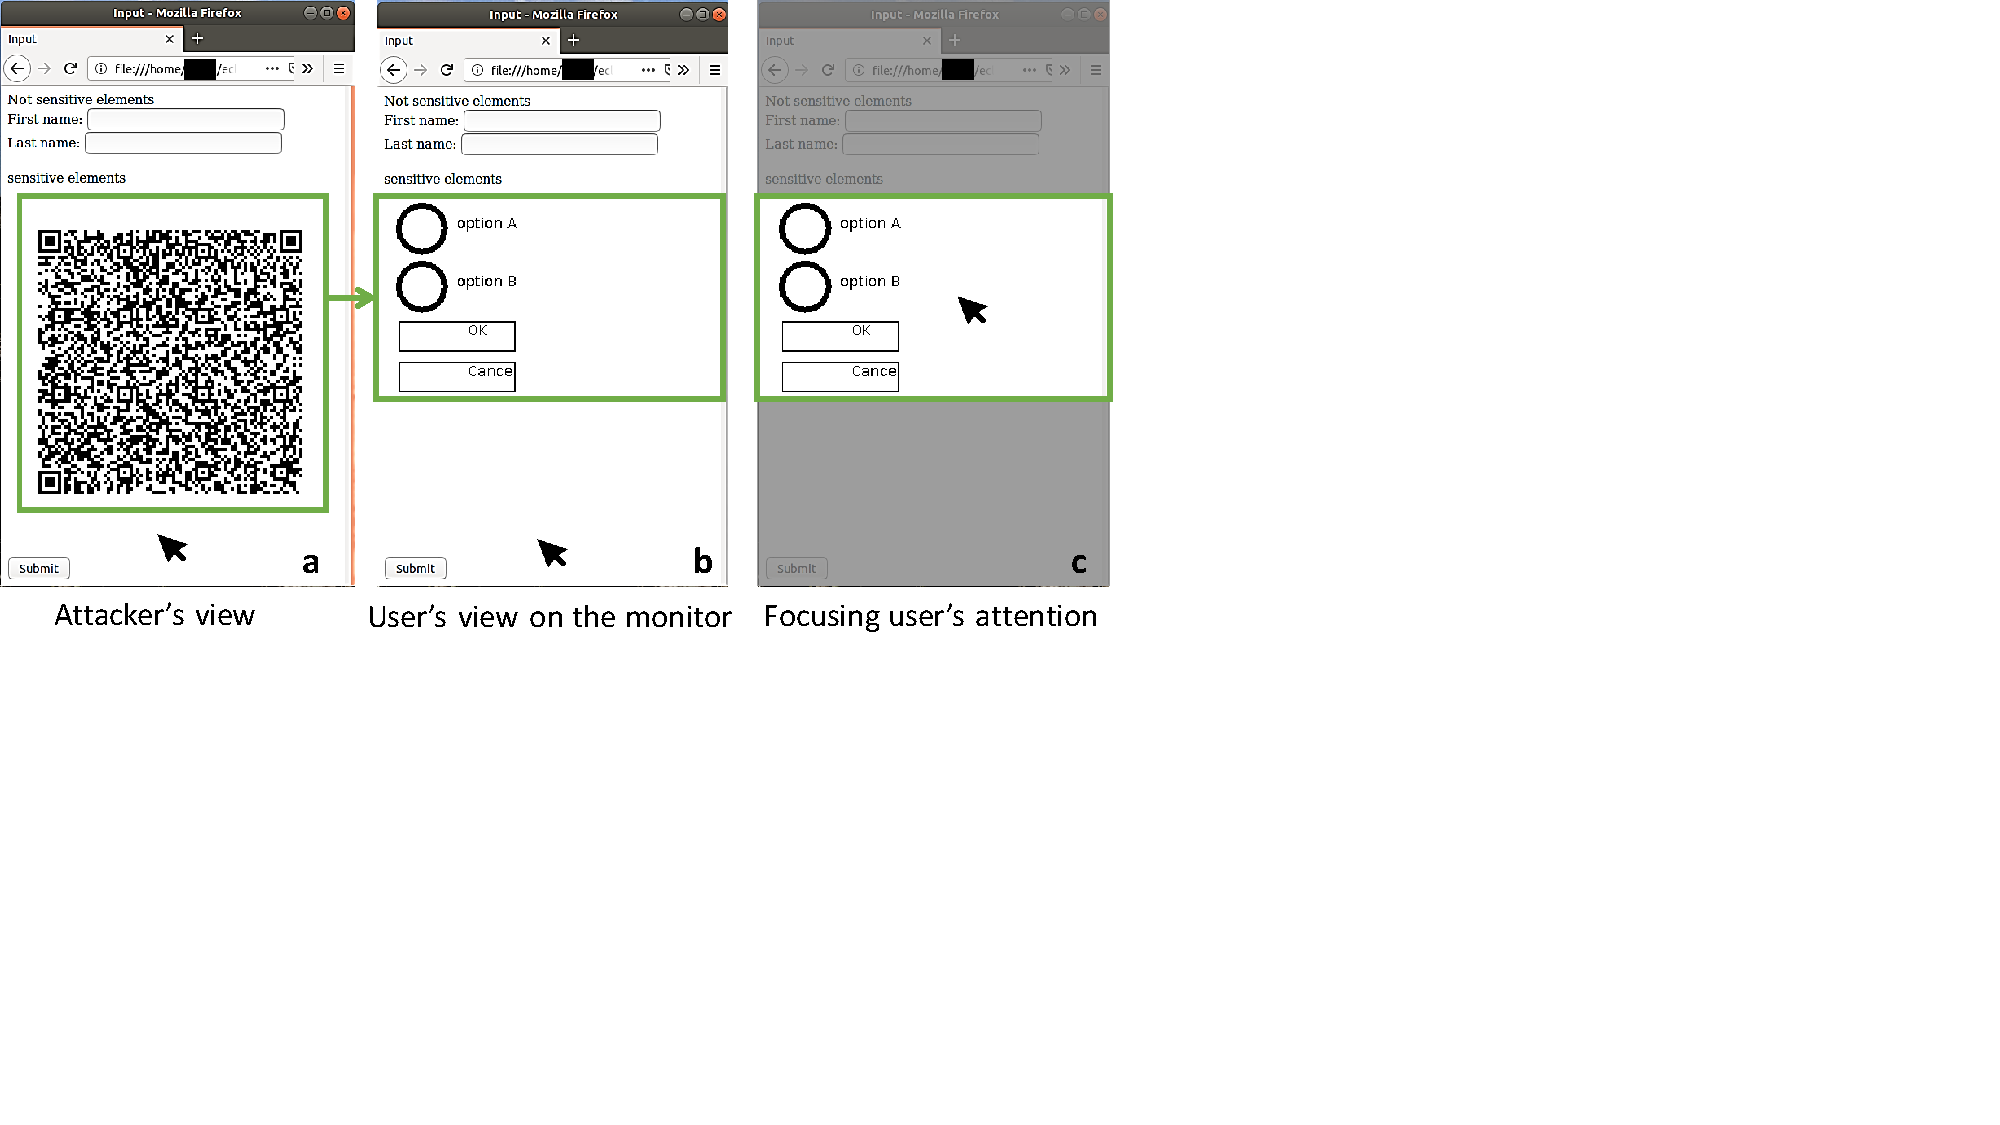
\includegraphics[trim={0 8cm 15cm 0}, clip, width=\linewidth]{overlayScreenShot_new.pdf}
\caption{\textbf{\name's high-level approach} shows that the \device generates UI overlay to protect IO integrity and confidentiality. a) The attacker only sees the non-protected UI elements, and the protected form is encrypted and encoded (in our case, the \device could decode a QR code and decrypt). b) shows the \device generated form overlay that is hidden from the host. The protected part of the screen provides integrity and confidentiality of all user IO. c) shows that the \device dims out (lightbox) the rest of the screen when the user moves her mouse pointer over the protected region to focus user attention.}
\spacesave
\label{fig:screenshot_1}
\end{figure}

\name is build upon the security requirements and functional properties that are described in Section~\ref{goals}. %\name achieves IO integrity and confidentiality by leveraging an external trusted component that we call \device (refer to Figure~\ref{fig:approachOverview}). 
%In our implementation, \device is realized as an external, low-TCB hardware that uses off-the-shelf components and \device is easy to integrate with legacy systems - providing \emph{easy deployment}. Figure~\ref{fig:approachOverview} illustrates the system configuration. \device sits between IO peripherals and the host system. It intercepts all keyboard and mouse events. Also, it can intercept \& overlay on the display signal. 
\device is active only when the user visits sensitive web applications that require \name security.
Initially, the remote server signs and delivers the sensitive UI elements to the host in a format that is understandable by \device. Next, the host transfers the sensitive UI to \device, and the \device verifies the signature to prevent manipulations by the host. As seen in a running example depicted in Figure~\ref{fig:screenshot_1}, the \device then renders the UI with sensitive elements into an overlay on top of the HDMI frame received from the host. Note that the host cannot access or modify the overlay generated by the \device. Also, the overlay covers only a part of the screen, allowing the other feature-rich content on the webpage to run unmodified. Therefore, this ensures that sensitive UI elements are presented to the user as expected by the remote server -- \emph{output integrity}. For the overlay, we use QR-codes to transfer data from the host to the device because we avoid using extra software/hardware for a separate channel, and it is easy to visualize.

When the user interacts (types or moves the pointer) with the overlay, \device does not forward any event from the keyboard or the mouse to the host. The interaction is maintained solely by \device, which renders on-screen user inputs and therefore offers a user experience that is identical to a typical one as if the \device is not present. The user click on the \emph{submit} button triggers the submission procedure, which consists of the \device signing the user inputs and sending to the server. Note that the text fields of the form and the \emph{submit} button are inside the overlay which is inaccessible by the host, hence the attacker cannot execute the early form submission or clickjacking attacks. Finally, the server verifies the signature of \device to guarantee that the host has not altered the data. Therefore, the \device ensures \emph{input integrity} for all \emph{modalities} of input.

For integrity guarantees, \name uses well-known user attention focusing mechanisms. Unlike systems like Fidelius, these mechanisms do not introduce any cognitive load to the users as \name does not rely on multiple security indicators. Mechanisms such as lightbox aid the user to distinguish the \device overlay on the screen from the rest. Thus, the untrusted host cannot trick the user into following malicious instructions when the user interacts with sensitive UI elements. Also, the host cannot observe sensitive data on the overlay because it does not have access to it. In the case where confidentiality is required, the user manually triggers SAS, such as the lightbox by pressing specific keys.

%Note that the lightbox technique is not the only way to capture the \emph{user attention}, e.g., freezing the untrusted part of the screen is another approach~\cite{huang2012clickjacking}. 
%To minimize user habituation and actively inform the user about the protected overlay, \device activates the user attention mechanism (the lightbox) automatically when the mouse pointer is over the overlay, or the user starts typing to a sensitive text field.
 


